%
%	TSD 2017
%	LaTeX Template for Camera-ready Version
%
%	Rel. 2013-05-20 by Ivan Habernal (habernal@kiv.zcu.cz)
%	Rel. 2014-11-21 by Kamil Ekstein (kekstein@kiv.zcu.cz)
%   Rel. 2015-02-23 by Pavel Kral    (pkral@kiv.zcu.cz)
%	Rel. 2017-02-06 by Kamil Ekstein (kekstein@kiv.zcu.cz)
%
%	Based upon Springer's LNCS series template.
%
\documentclass[runningheads,a4paper]{llncs}
\usepackage{dirtree}
\usepackage[nolist,nohyperlinks]{acronym}
\usepackage{times}
\usepackage{amssymb}
\setcounter{tocdepth}{3}
\usepackage{graphicx}
\usepackage{acronym}
\usepackage{url}
\usepackage[colorlinks]{hyperref}
\usepackage[utf8]{inputenc}
\usepackage{floatrow}
\usepackage{subfigure} 
\usepackage[spanish]{babel}
\selectlanguage{spanish}
\usepackage[utf8]{inputenc}
\floatsetup[table]{capposition=top}

\newfloatcommand{capbtabbox}{table}[\captop][\FBwidth]

\newcommand{\keywords}[1]{\par\addvspace\baselineskip
\noindent\keywordname\enspace\ignorespaces#1}

% TSD2017: Put your e-mail addresses here
\urldef{\mailsa}\path|a20133303@pucp.edu.pe|
\urldef{\mailsb}\path|meryalis@hotmail.com|
%\urldef{\mailsc}\path|other_mails_if_needed|    
%gvalderrama, msobrevilla pucp.edu.pe
\begin{document}

% TSD 2017: Put your title here (please, use capitalization, see e.g.
% http://en.wikibooks.org/wiki/Basic_Book_Design/Capitalizing_Words_in_Titles)
\title{Factores desencadenantes de una  Enfermedad Renal Crónica en pacientes con diagnóstico de Diabetes}

\titlerunning{Estudio de los Factores Desencadenantes de Una  Enfermedad Renal Crónica en Pacientes con Diagnóstico de Diabetes}

\author{Gregory César Valderrama Vilca\inst{1} Meryhelen Alisson Torres Vargas\inst{2}}
\authorrunning{Gregory Valderrama Vilca y Meryhelen Alisson Torres Vargas}


\institute{Escuela de Posgrado, Maestría en Estadística \\ Pontificia Universidad Católica del Perú \\
% TSD 2017: optional url
%\url{abc} \\
\mailsa\\
% TSD 2017: For authors from different institutions, add 2nd institution, etc.
\and
Hospital Guillermo Almenara \\
% Affiliation2, Institute2, Address \\
% \url{www.website.org} \\
\mailsb\\
}


% TSD 2017: Put all authors' names to the proceeding index (surname, first name)
\index{Valderrama Vilca, Gregory}
%\index{Torres Vargas, Meryhelen}

\toctitle{} \tocauthor{}

\maketitle

%
%
%	TSD2017 SUBMISSION TEXT
%
%
\begin{abstract}

El presente es un estudio realizado sobre los datos de 30 pacientes, con el diagnóstico de Diabetes Mellitus tipo 2, hospitalizados en la Unidad de Pie Diabético del Hospital Nacional Guillermo Almenara Irigoyen. \footnote{Disponible en https://es.wikipedia.org/wiki/Hospital\_Guillermo\_Almenara\_Irigoyen accedido en Abril 2018 }

Los datos fueron recopilados en los meses de enero a marzo del 2018, con el fin de detectar patrones en los datos y que estos ayuden al equipo médico del hospital. Primero nos enfocamos en explicar el comportamiento de la \ac{TFG} (medida del funcionamiento de los riñones) por ser un factor que puede llevar a la pérdida de la función renal y acarrear complicaciones graves para los pacientes. Posteriormente nos enfocaremos en explicar los factores que podrían estar asociados a que  un paciente con el diagnóstico de Diabetes Mellitus  desarrolle como complicación tardía: Pie Diabético de  tipo isquémico o Pie diabético de tipo Neuropático y de esta manera prevenir estas complicaciones,conociendo los factores intrínsecos y ambientales asociados. 


\keywords{ Tasa de Filtración Glomerular, Pie diabético, tratamiento, evolución.}

\end{abstract}

\section{Introducción}

La diabetes va a ser una de las mayores crisis de salud en el año 2030. Se espera que para este tiempo se haya incrementado en un 54\%, alcanzando en EEUU, los 54 millones de pacientes, con una tasa de mortalidad de 385 mil personas anualmente y costos a la sociedad por 622 mil millones de dólares \cite{rowley2017diabetes}. 

Las complicaciones relacionadas con los pies en un diabético son comunes y se estima que entre un 20\% y 40\% desarrollara algún daño nervioso o neuropatía y un 5\% desarrolla úlceras \cite{kumar1994prevalence}. 

Dichos números exigen que las autoridades sanitarias centren sus esfuerzos en combatir esta enfermedad incluyendo al pie diabético. Y sin duda es importante desarrollar modelos que den la capacidad de predecir las posibles complicaciones en los pacientes, lo que será de mucha utilidad para aliviar el sufrimiento que provoca esta enfermedad.

El objetivo del trabajo es analizar las variables relacionadas a la \ac{TFG} y tipo de Pie diabético desarrollado, en la muestra de 30 de pacientes con el diagnóstico de  Diabetes Mellitus,  hospitalizados en el  Hospital Nacional Guillermo Almenara Irigoyen. \footnote{Disponible en https://es.wikipedia.org/wiki/Hospital\_Guillermo\_Almenara\_Irigoyen accedido en Abril 2018 }. Evaluando las variables de:  edad, sexo, estado civil, tiempo de diagnóstico de diabetes, tratamiento para la diabetes, peso, talla, índice de masa corporal, hipertensión arterial, hemoglobina, hemoglobina glicosilada, triglicéridos, colesterol, colesterol HDL, albúmina, \ac{BUN}, urea, creatinina.


\section{Trabajos Relacionados}

A nivel individual, los principales factores de riesgo para Enfermedad Renal Crónica son la diabetes mellitus, \ac{HTA}, edad avanzada, historia familiar de la enfermedad, entre otros. Según \cite{hamada2018multiple}, la prevalencia de ERC en pacientes con diabetes está entre 4.2\% y 17.9\% (estadios ERC 3-5) en Países europeos. No obstante, en el estudio realizado por \cite{guenzani2018there}, donde se evaluó un total de 32.616 pacientes diabéticos, reclutados de 997 hospitales. De los participantes, el 35.4\% eran pacientes con ERC. 

El BUN es un parámetro de función renal, por lo que estos resultados se encuentran validados por múltiples estudios.  Así, \cite{tanaka2017impact} realizó un estudio donde evaluó la asociación entre el nivel de BUN/Creatinina y la supervivencia en pacientes con enfermedad renal crónica terminal en  hemodiálisis; evaluó un total de 3,401 pacientes en hemodiálisis, los cuales  fueron seguidos prospectivamente durante 4 años. La asociación entre BUN/creatinina con la supervivencia global se analizó utilizando un modelo de regresión de Cox. Durante un período de seguimiento de 4 años, 545 pacientes murieron por cualquier causa y 582 experimentaron eventos cardiovasculares mayores, 392 con enfermedad coronaria, 114 con muerte relacionada con infección, 77 con accidente cerebrovascular hemorrágico, 141 con accidente cerebrovascular isquémico y 107 con muerte por cáncer. Cada 1 aumento en el nivel de BUN/creatinina se asoció significativamente con un mayor riesgo de mortalidad por todas las causas (cociente de riesgos instantáneos [HR] 1,07; intervalo de confianza [IC] del 95\%: 1,03-1,12), CC (CRI 1,08; IC del 95\%: 1,02-1,14) y muerte relacionada con infección (CRI 1.11, IC 95\% 1.02-1.21). No hubo evidencia de una asociación significativa entre BUN/creatinina y muerte por cáncer e incidencia de accidente cerebrovascular. Un alto BUN/creatinina se asoció significativamente con un mayor riesgo de mortalidad por cualquier causa, muerte relacionada con infección y mayor incidencia de enfermedad coronaria en pacientes en hemodiálisis. Por lo que se sugiere ampliar el estudio evaluando la relación BUN/creatinina.

\cite{yun2018obesity} evaluaron a 1.940 participantes del Estudio Cohorte de Corea,  Pacientes con Enfermedad Renal Crónica cuyos predictores fueron:  Obesidad y anormalidad metabólica  definida por  5 componentes: hipertensión, nivel de glucosa en ayunas mayor a 125 mg / dl o la presencia de diabetes tipo 2, nivel de triglicéridos> 150 mg / dL o el uso de fármacos hipolipemiantes, nivel de colesterol HDL \≤ 40 mg / dl en hombres y \≤ 50 mg / dl en mujeres, y nivel de proteína C reactiva de alta sensibilidad> 1 mg / l.  
Durante un seguimiento promedio de 3.1 años, la obesidad y la anomalía metabólica se asociaron significativamente con 1,41 veces (IC 95\%, 1,08-1,83, P = 0,01) y 1,38 veces (IC 95\%, 1,03-1,85; P = 0,03 ) aumento del riesgo de resultados renales adversos, respectivamente. Asimismo,  aquellos con obesidad y anomalías metabólicas tenían un mayor riesgo de progresión de la ERC (CRI, 1.53, P = 0.03).  Sin embargo no existen estudios al momento que establezcan una relación directa entre colesterol total y ERC; por lo que este dato requiere mayor estudio.

\section{Descripción de Datos}

El estudio se realizó sobre una muestra de 30 pacientes de la Unidad de Pie Diabético del Hospital Nacional Guillermo Almenara Irigoyen, los cuales fueron recopilados en los meses de enero a marzo del año 2018.

Se define como variable respuesta o dependiente la \ac{TFG} que es de tipo continua y el tipo de pie diabético desarrollado por el paciente, que puede tomar un valor categórico de isquémico o neuropático en la Figura
\ref{fig:categorico_descriptivo}.  

Del primer análisis descriptivo, en la Figura \ref{fig:continuo_descriptivo}, podemos identificar algunos valores extremos, principalmente en BUN y IMC, estos valores anómalos deben ser enviados al equipo médico para su validación. .

Se definen como variables explicativas o independientes a continuación: 

\begin{itemize}

\item \textbf{Sexo}, variable cualitativa, que indica el sexo de una persona, puede ser masculina o femenina.

\item \textbf{Edad}, variable cuantitativa de carácter continuo, que indica la edad de una persona en años.

\item \textbf{Estado civil}, variable cualitativa, que indica si una persona está casada o soltera.

\item \textbf{Peso}, variable cuantitativa de carácter continuo, que indica el peso de una persona en kilogramos.


\item \textbf{Talla}, variable cuantitativa de carácter continua, que indica la talla de una persona en metros.

\item \textbf{Índice de masa corporal}, variable cuantitativa de carácter continua, que indica la relación entre el peso y la talla de una persona. Índice de masa corporal  se calcula dividiendo los kilogramos de peso por el cuadrado de la estatura en metros (IMC = peso [kg]/ estatura [m2]) 

\item \textbf{\ac{HTA}}, variable cualitativa binaria, que indica si la persona tiene o no el diagnóstico de hipertensión arterial (HTA) asociado al diagnóstico de  diabetes mellitus.

\item \textbf{Tiempo de diagnóstico de diabetes mellitus}, variable cuantitativa de carácter continua,  que indica el tiempo en años, que una persona lleva con el diagnóstico de diabetes mellitus.

\item \textbf{Tratamiento recibido para la diabetes mellitus}, variable cualitativa, que indica el tipo de tratamiento que lleva el paciente previo su hospitalización, con los valores de: Antidiabéticos orales (ADO), insulina o  ninguno.

\item \textbf{ \textit{Creatinina}}, variable cuantitativa continua, que indica el parámetro de la función renal, con un valor normal menor a 1. La creatinina es un producto de desecho que proviene de la actividad muscular. Cuando los riñones están funcionando correctamente, eliminan la creatinina de la sangre. A medida que la función renal disminuye, los niveles de creatinina en sangre, se elevan.

\item \textbf{Hemoglobina}, variable cuantitativa continua, usada comúnmente para detectar anemia, un nivel anormalmente bajo de glóbulos rojos en el cuerpo; dado que la hemoglobina es una proteína de los glóbulos rojos que lleva oxígeno de los pulmones al resto del cuerpo. Los valores normales van entre 13,3 y 18 g/dl en hombres; 11,7 a 15,7 g/dl en mujeres.


\item \textbf{\ac{BUN}}, variable cuantitativa continua, que indica  la cantidad de nitrógeno circulando en forma de urea en el torrente sanguíneo. La urea es una sustancia secretada a nivel del hígado, producto del metabolismo proteico, a su vez, es eliminada a través de los riñones. Por lo que el BUN es un indicador de la función renal. El rango normal es de 9 a 23 mg/dL.

\item \textbf{UREA}, variable cuantitativa continua, que  es el producto resultante de la degradación de las proteínas llevada a cabo por el hígado. Filtrada por los riñones, la urea se elimina a través de la orina, como un residuo del organismo. Un cantidad elevada de urea en la sangre puede indicar un daño renal. El rango normal es de 15 a 45 mg/dL.

\item \textbf{ALBUMINA}, variable cuantitativa continua, es una proteína que se encuentra en gran proporción en el plasma, siendo la principal proteína de la sangre, y una de las más abundantes en el ser humano. Se sintetiza en el hígado. Es un parámetro que estima la función hepática, renal y nutricional. El rango normal es de 3.2 a 4.8 gramos por decilitro (g/dL).

\item \textbf{TRIGLICERIDOS}, variable cuantitativa continua, son lípidos que se encuentran en determinados alimentos y también se producen en el hígado. Los triglicéridos circulan en la sangre mediante unas lipoproteínas que se producen en el intestino y en el hígado y se transportan a los tejidos donde se utilizan como una reserva de energía para cubrir las necesidades metabólicas de los músculos y el cerebro. Las causas más frecuentes de aumento de los triglicéridos son el sobrepeso / obesidad, el exceso de alcohol, la inactividad física, una dieta muy alta en hidratos de carbono (60\% o más de las calorías) especialmente si son refinados y fumar.  Normal: menos de 150 mg/dL. Limítrofe alto: 150 a 199 mg/dL. Alto: 200 a 499 mg/dL. Muy alto: 500 mg/dL o superior.

\item \textbf{\ac{COL}}, variable cuantitativa continua,  es una sustancia similar a la grasa e indispensable para la vida. Se encuentra en las membranas celulares de nuestros organismos, desde el sistema nervioso al hígado y al corazón. El cuerpo necesita colesterol para fabricar hormonas, ácidos biliares, vitamina D, y otras sustancias. Sin embargo, el aumento del colesterol en la sangre y su depósito en las arterias puede ser peligroso y producir ateroesclerosis (estrechamiento o endurecimiento de las arterias por depósito de colesterol en sus paredes). Una parte importante del colesterol de nuestro organismo se produce en el hígado. El resto es aportado a través de la dieta y del colesterol presente en la bilis, parte del cual se vuelve a absorber en el intestino. El nivel de colesterol normal es inferior a 200 mg/dl. Niveles cercanos al límite son 200 a 239 mg/dl y niveles por encima de 240 mg/dl se considera alto.

\item \textbf{HDL}, variable cuantitativa continua. Las siglas HDL provienen de la abreviatura en inglés de las palabras lipoproteínas de alta densidad (high density lipoproteins). Las HDL son unas partículas de muy pequeño tamaño compuestas por grasas (sobre todo colesterol y fosfolípidos) y una proporción alta de proteínas (sobre todo una proteína que se llama apolipoproteína A-1).  Las HDL evitan que el colesterol se deposite en exceso en el interior de las arterias y de este modo previenen la arteriosclerosis que es la causa del infarto de miocardio, la angina de pecho y otras enfermedades, como los infartos cerebrales. Cuanto mayor es la cantidad de HDL, más grande es la protección frente a la arteriosclerosis. Los valores normales oscilan entre 40 y 60 mg/dl. 

\item \textbf{\ac{GLI}}, variable cuantitativa continua, GLI (Hemoglobina glicada) se encuentra directamente relacionada conl promedio de glucosa sérica, porque la glicación  de la hemoglobina es un proceso relativamente lento, no-enzimático, que sucede durante los 120 días de la vida media del eritrocito y que termina en la glicación irreversible de la hemoglobina de los glóbulos rojos hasta su muerte,  por lo que la GLI refleja la glucemia media del individuo en los tres a cuatro meses previos a la toma de la muestra, estimando el control de la glucemia en ese periodo de tiempo. 

\item \textbf{\ac{TFG}} , variable cuantitativa continua dependiente, que sirve para determinar el grado de insuficiencia renal. La tasa de filtración glomerular es la mejor medida de la función renal. Es el número que se utiliza para determinar la etapa de la enfermedad renal de una persona. Para calcular la \ac{TFG}, se utiliza la fórmula CDK EPI que tiene en cuenta la edad de la persona, la raza, el sexo y la creatinina sérica.

\end{itemize}

\begin{figure}[!ht]
\centering
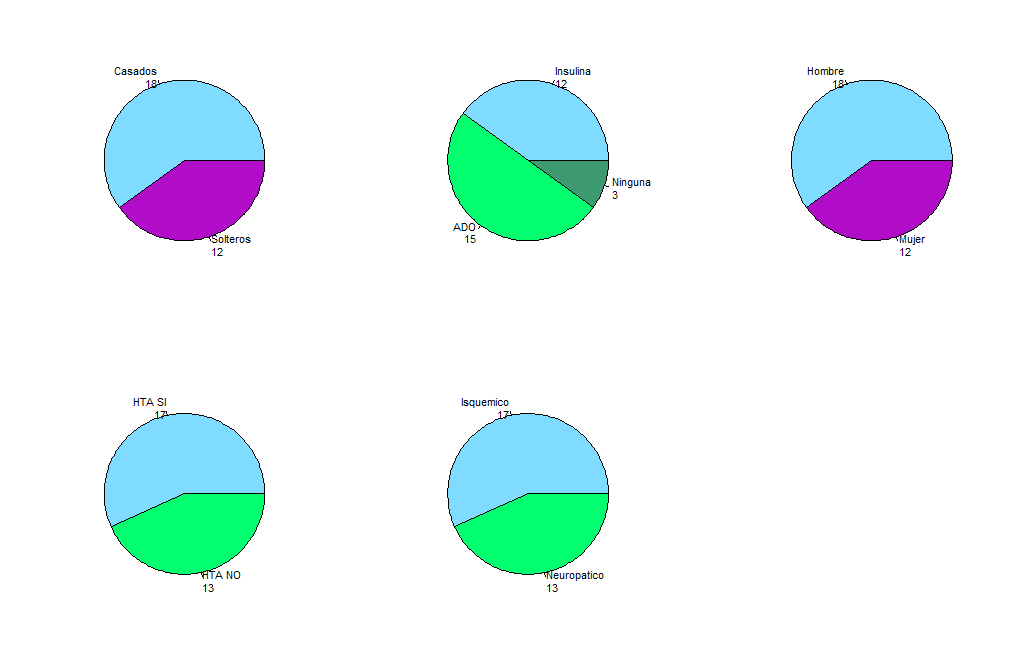
\includegraphics[scale=0.5]{imagesv2/categoricas.png}
\caption{Variables Categoricas }
\label{fig:categorico_descriptivo}
\end{figure}

\begin{figure}[!ht]
\centering
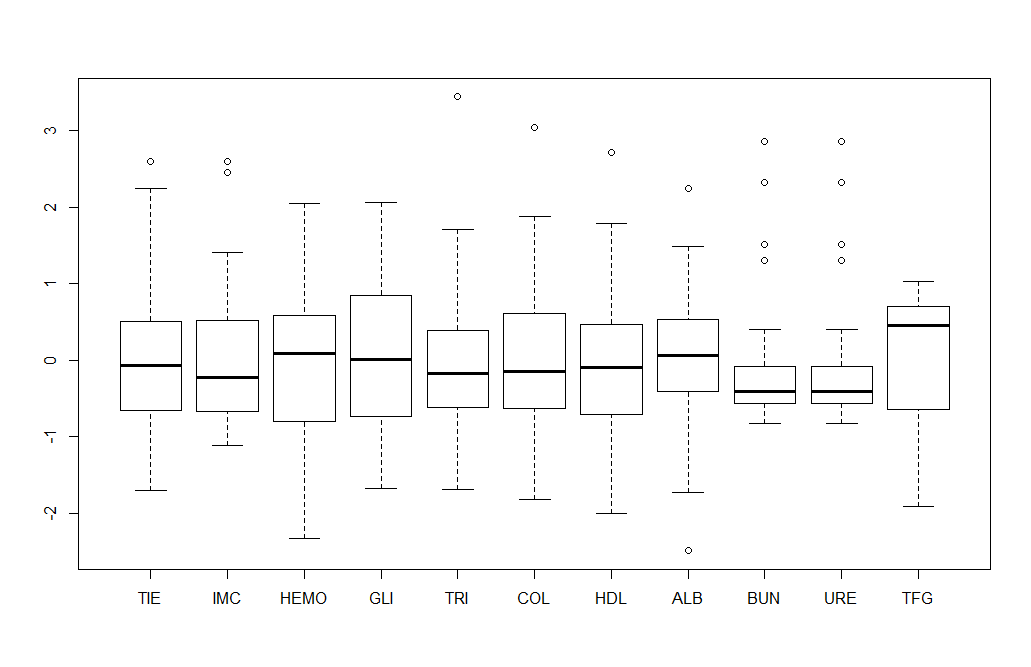
\includegraphics[scale=0.4]{imagesv2/boxplotscaled.png}
\caption{Box Plot Variables Continuas}
\label{fig:continuo_descriptivo}
\end{figure}



\section{Análisis  de  Correlación Tasa de Filtración Glomerular}

Cuando se estudia la correlación de variables, es usual recurrir al llamado análisis de la correlación. En las seccion anterior utilizamos primero un diagrama de cajas para mostrar la distribución de los datos estandarizados, después el índice de correlación de Pearson y los diagramas de dispersión para analizar la correlación entre las variables independientes que son el Tiempo de diagnóstico, IMC, Hemoglobina, Triglicéridos, Colesterol, HDL, Albúmina, BUN, Urea. 


A continuación: el índice de Pearson para correlacionar y diagramas de dispersión, en la Figura \ref{fig:independientes_correlacion}.


\begin{figure}[!ht]
\centering
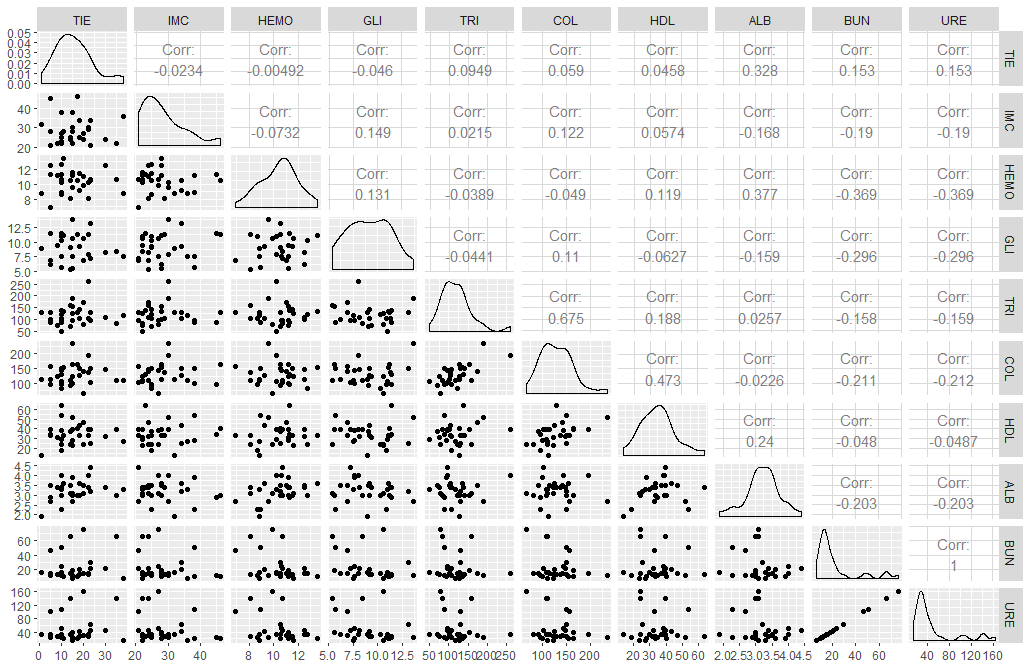
\includegraphics[scale=0.4]{imagesv2/pearsondispersion.png}
\caption{Variables Independientes Correlacion}
\label{fig:independientes_correlacion}
\end{figure}

Podemos detectar una correlación perfecta entre la variable BUN y UREA lo que nos informa de que hay colinealidad en dichas variables explicativas, lo cual tiene sentido pues ambas variables hacer referencia a un indicador común; por lo que a partir de este punto continuamos con una de ellas, BUN, porque a diferencia de la creatinina, si es influenciado por varios factores. Problemas cardíacos, la deshidratación y una dieta con alto contenido de proteínas pueden elevar falsamente el resultado de la medición del nitrógeno ureico. No obstante, el nitrógeno ureico tiene una ventaja: puede ayudar a detectar un daño renal más tempranamente que la creatinina. Además nos permitiría diferenciar entre  Insuficiencia Renal "renal o prerrenal".


%, de la siguiente manera: BUN/Cr (S) relación > 20 porcentaje (> 0.2 fracción) indica causa prerrenal. BUN/Cr (S) relación < 10 percentaje (< 0.1 fracción) indica causa renal.

Garantizada la no colinealidad de las variables explicativas, analizamos la correlación entre  éstas y la variable dependiente \ac{TFG}, en la Figura \ref{fig:dependiente_correlacion}.


\begin{figure}[!ht]
\centering
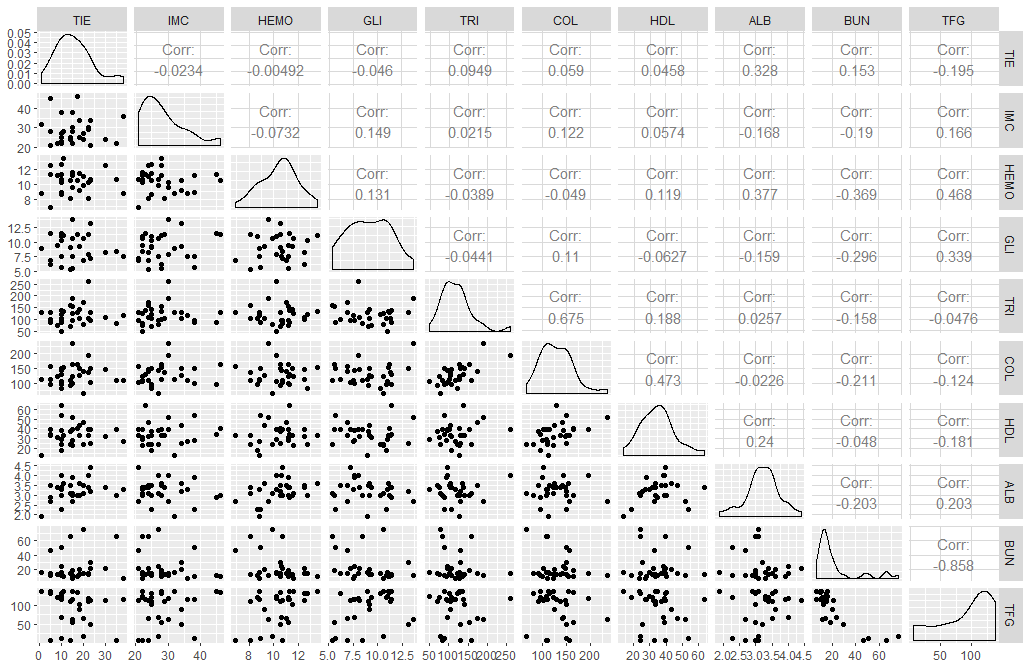
\includegraphics[scale=0.4]{imagesv2/correlaciontfg.png}
\caption{Variables Continuas Dependiente e Independientes Correlacion}
\label{fig:dependiente_correlacion}
\end{figure}

La correlación puede ser positiva o negativa pero debe indicar un valor cercano a 1 o -1, podemos visualizar que la variable con una alta correlación es \ac{BUN} (-0.858), adicionalmente analizaremos la correlación de la variable \ac{HEMO} (0.468) y \ac{GLI}  (0.339). Por lo mismo podemos descartar una correlación con el tiempo de diagnóstico, índice de masa corporal, los triglicéridos, el colesterol, HDL y albúmina.

El análisis de regresión lineal nos permite desarrollar una ecuación lineal que explique el efecto de las variables independientes (\ac{BUN}, \ac{HEMO}, \ac{GLI} ) sobre la variable dependiente objetivo \ac{TFG}. Utilizando la técnica de mínimos cuadrados determinamos una ecuación que minimice las distancias verticales entre los valores reales de TFG y los valores pronosticados por la ecuación lineal. Al terminar podremos explicar mejor cual es la relación entre las variables y pronosticar un comportamiento para nuevos valores en las variables independientes.

Primero analizaremos el efecto de la variable BUN sobre \ac{TFG}, mediante una regresión lineal simple o de una sola variable.

\begin{figure}[!ht]
\centering
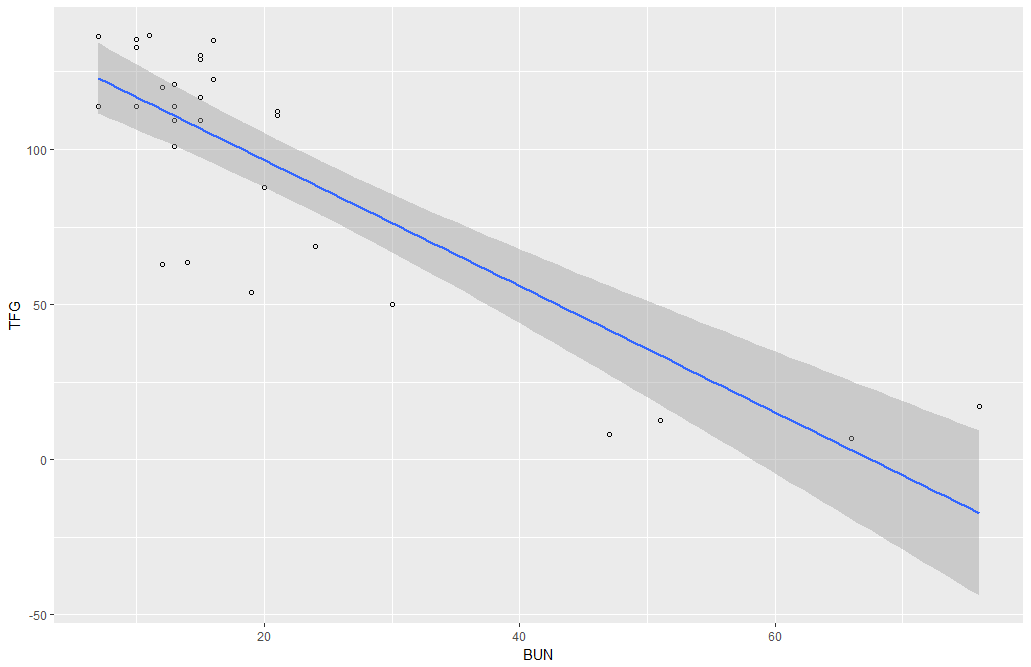
\includegraphics[scale=0.4]{imagesv2/lineal_tfg_bun.png}
\caption{Regresion Lineal TFG explicada por BUN}
\label{fig:lineal_tfg_bun}
\end{figure}

Nuestra primera regresión tiene un error estándar de 23.21 con 28 grados de libertad, el coeficiente de determinación (R cuadrado ajustado) es de 0.7267, lo cual indica que el 73\% del comportamiento de TFG se puede explicar por el comportamiento de BUN. El test de significancia (p-value) es menor a 0.05 por lo que podemos rechazar la hipótesis nula y por lo tanto la regresión es estadísticamente significativa. A continuacion analizamos el comportamiento de los residuos, en la Figura \ref{fig:lineal_tfg_bun_residuals}. 

\begin{figure}[!ht]
\centering
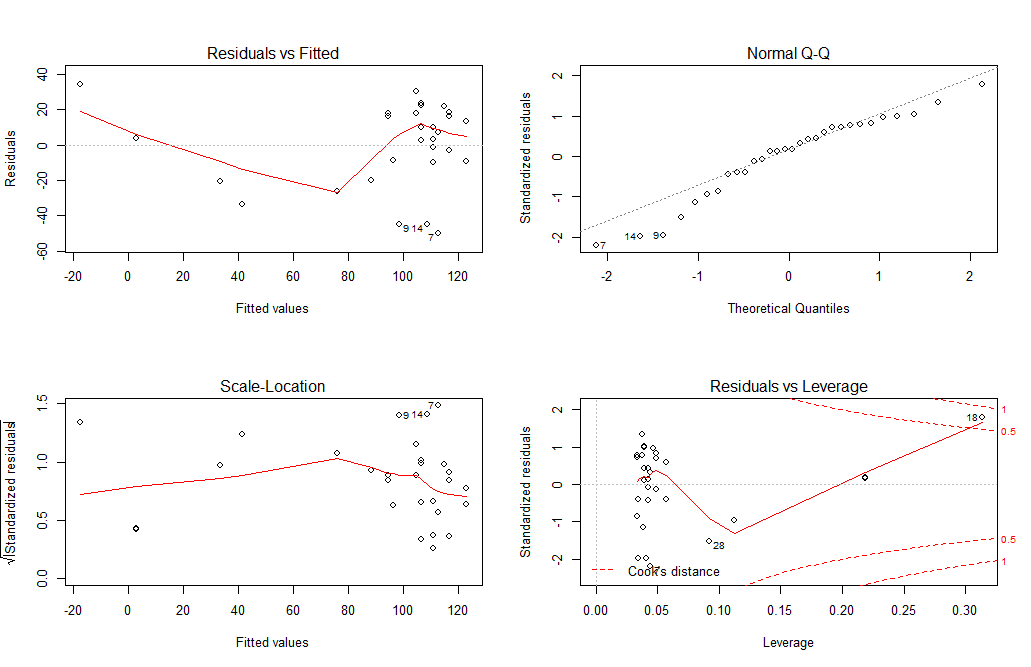
\includegraphics[scale=0.4]{imagesv2/lineal_tfg_bun_residuals.png}
\caption{Regresion Lineal TFG explicada por BUN, Residuos }
\label{fig:lineal_tfg_bun_residuals}
\end{figure}


Comprobamos el supuesto de normalidad de los residuos mediante un contraste de hipótesis de normalidad de Shapiro Wilk por tener menos de 50 muestras donde: 

H0 : los datos proceden de una distribución normal
 
H1 : los datos no proceden de una distribución normal

Con un p-valor de 0.04784 debemos rechazar la hipótesis nula y confirmar una distribución no normal para los errores por lo que nuestro modelo no puede explicar el comportamiento de la variable \ac{TFG}.

Comprobamos el supuesto de homocedasticidad mediante un contraste de hipótesis de Levene donde:

H0 : Varianza de todos los residuos son iguales
H1 : Al menos una varianza distinta entre los residuos 

Con un p-valor de 0.7723662 debemos aceptar la hipótesis nula y probamos que la varianza de los residuos es igual. Al no cumplir con los supuestos para una analisis de regresion lineal y a pesar de tener una alta correlación entre la variable BUN y TFG, nuestro modelo no puede explicar el comportamiento de la variable dependiente.

Un análisis similar se realizó con las variables \ac{HEMO} en la Figura  \ref{fig:lineal_tfg_hemo} y \ac{GLI} en la Figura \ref{fig:lineal_tfg_gli} que presentan los valores de correlacion mas importantes en nuestros datos, encontrando también que no superan el supuesto de normalidad de los residuos. Lo que significa que ninguna de estas variables puede explicar mediante un modelo lineal y por si sola el comportamiento de la variable \ac{TFG}.

\begin{figure}[!ht]
\centering
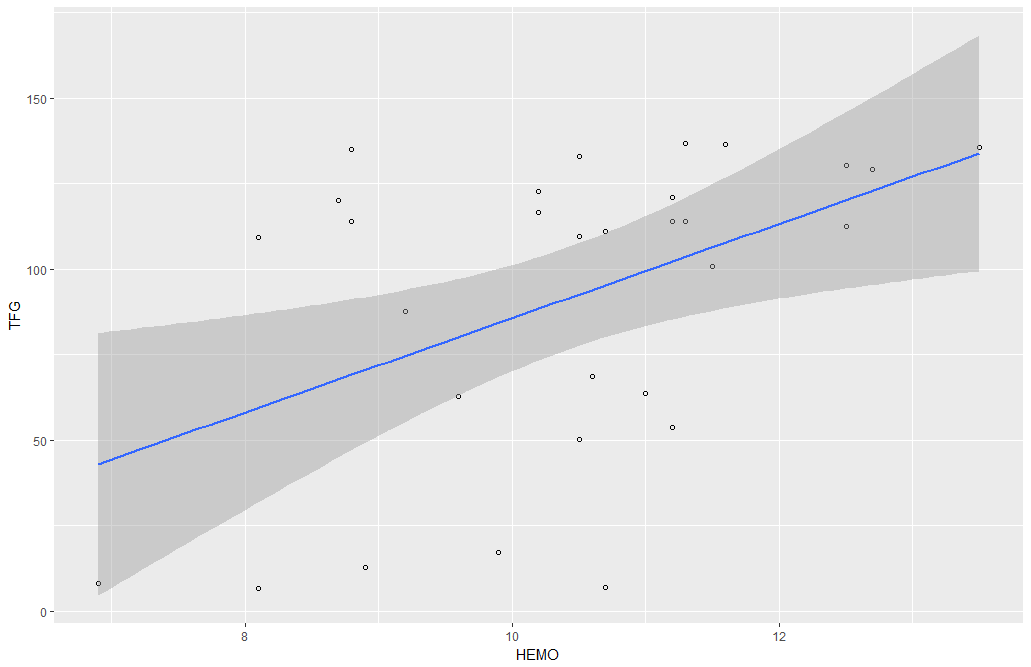
\includegraphics[scale=0.4]{imagesv2/lineal_tfg_hemo.png}
\caption{Regresion Lineal TFG explicada por HEMO  }
\label{fig:lineal_tfg_hemo}
\end{figure}

\begin{figure}[!ht]
\centering
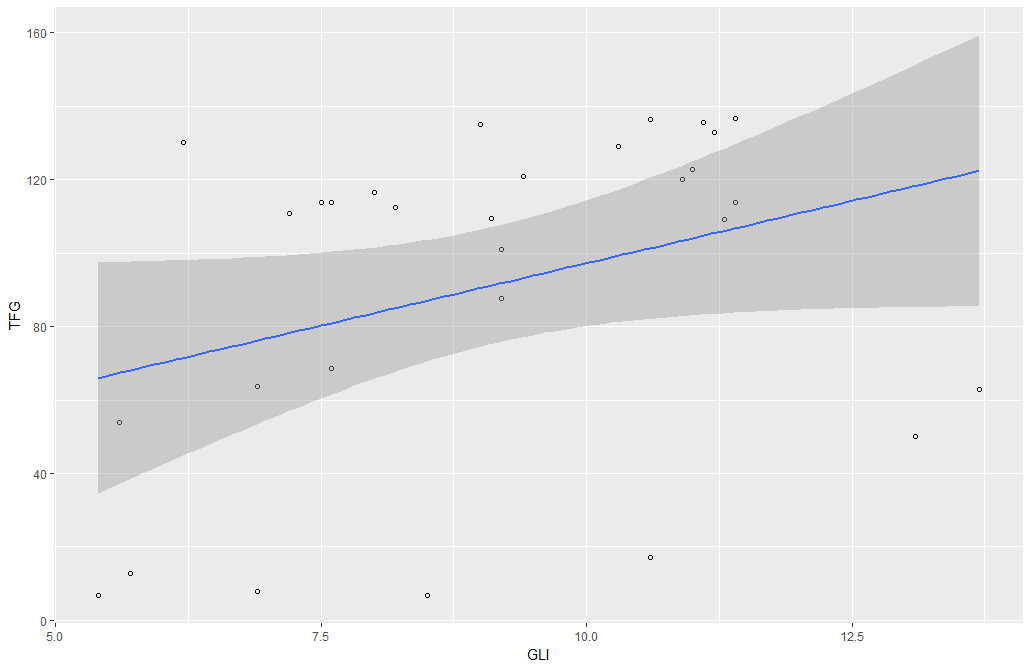
\includegraphics[scale=0.4]{imagesv2/lineal_tfg_gli.png}
\caption{Regresion Lineal TFG explicada por GLI  }
\label{fig:lineal_tfg_gli}
\end{figure}

A continuación utilizamos un modelo que incluya más de una variables explicativas para TFG, con este propósito utilizamos una búsqueda combinatoria conocida como “stepwise”, que nos permite evaluar automáticamente distintas combinaciones de regresores, utilizamos las técnicas de backward, forward y both; culminando todas con la misma sugerencia de variables BUN, COL, HDL y HEMO.  Dicho modelo tiene un p-valor menor a 0.5 y un explica el 83.8\% del comportamiento de TFG (R2 Ajustado).  Dicho modelo supera el test shapiro-wilk de normalidad con un p-valor de 0.6129 y supera el test de varianzas homogéneas con un test de Levene con un p-valor de 0.664.

\begin{figure}[!ht]
\centering
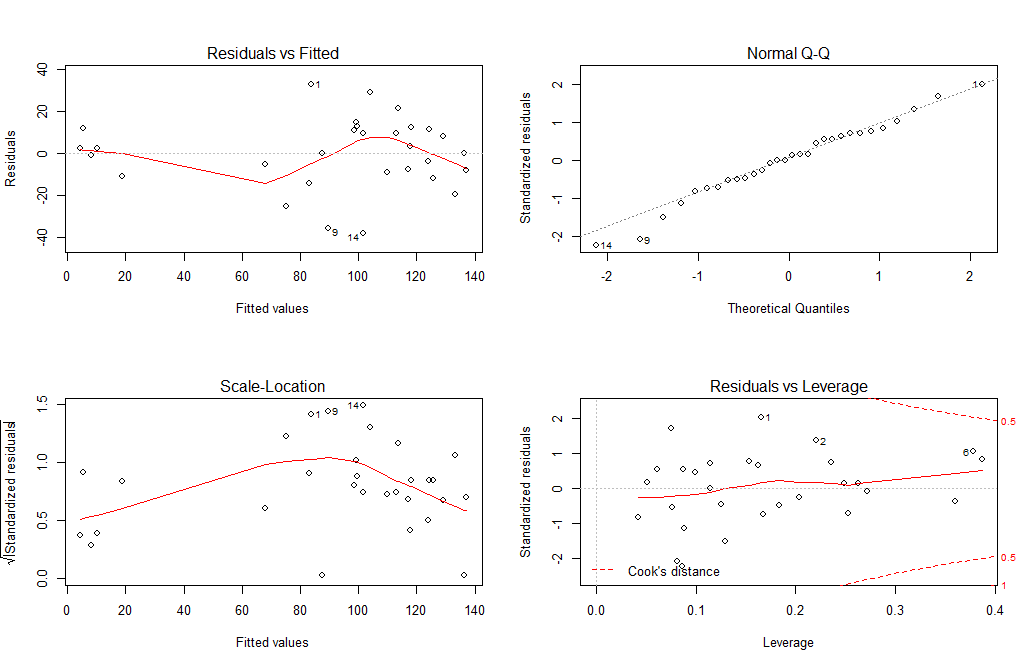
\includegraphics[scale=0.4]{imagesv2/lm_both_residuals.png}
\caption{TFG = BUN + COL + HDL + HEMO }
\label{fig:lm_both_residuals}
\end{figure}

Aunque nuestro modelo multivariado ha superado los supuestos de normalidad y homocedasticidad, es necesario minimizar el número de variables para así facilitar la interpretación y predictibilidad del modelo, por esta razón comparamos la bondad de nuestro modelo actual y la posibilidad de retirar alguna variable con poco significación mediante un análisis de la varianza (ANOVA).

Empezamos con la variable HDL cuyo p-value para el F-estadístico  es mayor a 0.05 por lo que presencia en el modelo puede ser no significativa. Al comparar ambos modelos, nuestro análisis ANOVA con p-valor de 0.1481  indica que no hay significativa entre ambos modelos y aunque nuestro error estándar para los residuos paso de 17.87 a 18.29, por esta razón retiramos la variable HDL de nuestro modelo. Nuestro nuevo modelo también supera el test de shapiro-wilk con 0.6755 and Levene con p-valor 0.68.

Evaluando la variable HEMO cuyo nuevo p-value para el F-estadístico pasó ha ser no significativo con 0.1279. Nuestro análisis ANOVA con p-valor de 0.1279 indica que no hay diferencia significativa entre un modelo que contenga la variable HEMO y uno que no. Al retirar dicha variable nuestro R2 ajustado a reducido un punto su efectividad a 82\% manteniendo un error estándar para los residuos y un nivel apropiado de significancia p-valor. Por esta razón y para simplificar el modelo explicativo retiramos del modelo la variable HEMO. 

Nuestro modelo que solo contempla las variables BUN y COL supera el test de shapiro-wilk para normalidad con un p-valor de 0.8943 y el test de Levene con un p-valor de 0.80. Como podemos apreciar en las siguientes gráficas.

\begin{figure}[!ht]
\centering
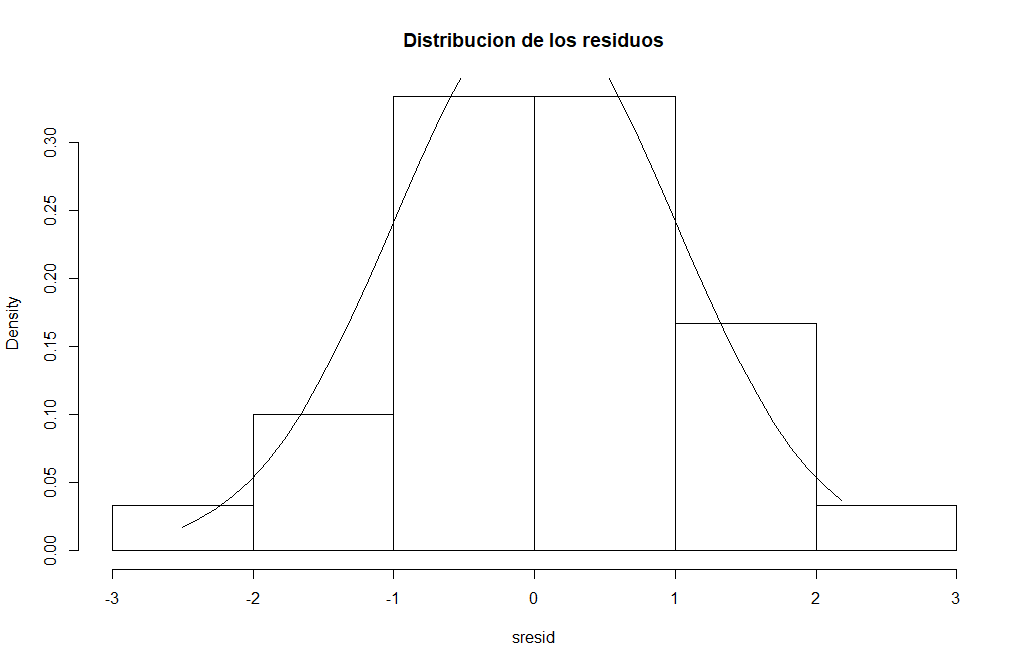
\includegraphics[scale=0.4]{imagesv2/lm_final_normal.png}
\caption{TFG = BUN + COLO , Residuos }
\label{fig:lm_both_residuals}
\end{figure}

Podemos visualizar la influencia de los valores extremos en nuestro modelo mediante el uso de la distancia de Cook explicado en la siguiente gráfica.

\begin{figure}[!ht]
\centering
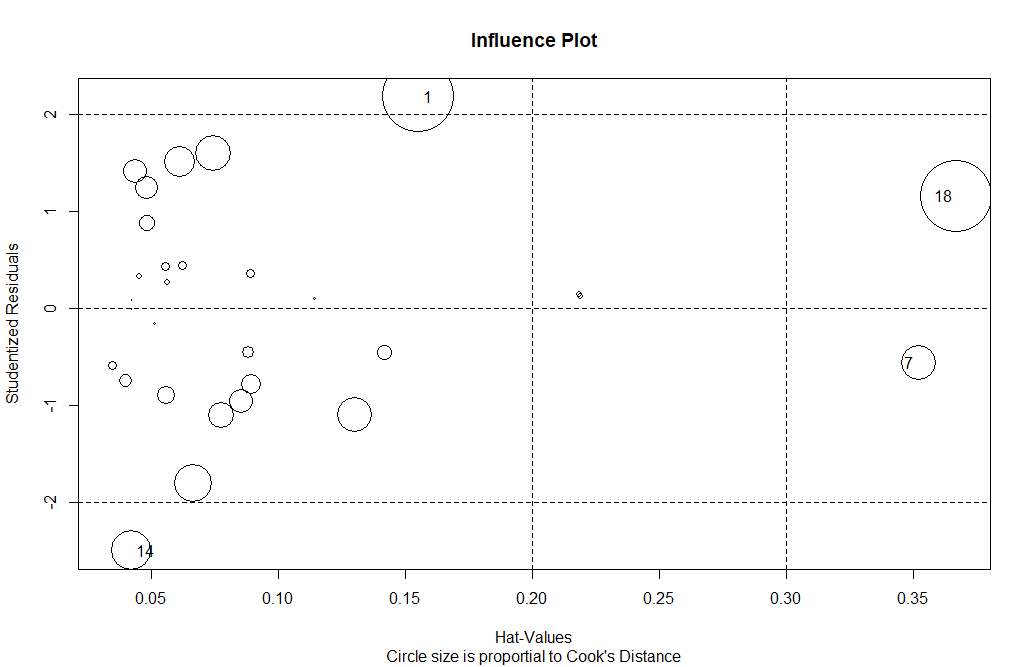
\includegraphics[scale=0.4]{imagesv2/influence_plot.png}
\caption{Grafico de influencia de los valores extremos en los residuos}
\label{fig:influence_plot}
\end{figure}


Por último debemos validar que los errores no estén correlacionados, debido a que si lo estuvieran podríamos subestimar el error estándar y causar que predictores que pensamos significativos, realmente no lo sean. Para esto utilizamos el test de Durbin Watson donde:

H0 : Significa que no hay correlación entre los residuos 

H1 : Los residuos están correlacionados

Nuestro modelo obtiene un p-valor de 0.34 por lo que aceptamos la hipótesis nula, no hay correlación en nuestros residuos.

Nuestro modelo entonces ha superado los supuestos de :

Los errores son independientes y no están correlacionados
No colinealidad entre las variables explicativas.
Normalidad en los residuos 
Homocedasticidad de varianza en los residuos 
 
Nuestro modelo explica el 82\% de la variable TFG, siendo los coeficientes de la variable BUN y COL -2.1925 y -0.4097 respectivamente, lo que indica que por cada unidad de variación positiva en la variable BUN podemos esperar una reducción de 2.1 puntos en la variable TFG por ejemplo.

\subsection{Análisis multivariado con variables categóricas}

Evaluamos la correlación que tienen las variables categorías de nuestros análisis con respecto al modelo multivariado desarrollado sobre las variables continuas BUN y COL.

Con respecto a la variable Sexo al introducir dicha variable en nuestro modelo nuestro análisis ANOVA indicó que no existe una diferencia significativa en la capacidad explicativa de nuestro modelo, por lo que concluimos que la variable sexo no implica relevancia al momento de explicar la variable TFG.

Con respecto a la variable Tratamiento mediante un análisis ANOVA no se encontró significancia en un modelo que incluya dicha variable categórica.

Con respecto a la variable Pie Diabético un análisis ANOVA encontró una significancia de un modelo que incluya dicha variable con respecto al modelo original con un p-valor de 0.029. 

Nuestro modelo explica ahora el 84\% del comportamiento de la variable TFG mantiene un error estándar de residuos de 17.44. A continuación las gráficas de residuos para el nuevo modelo, en la Figura \ref{fig:final_residuos}.


\begin{figure}[!ht]
\centering
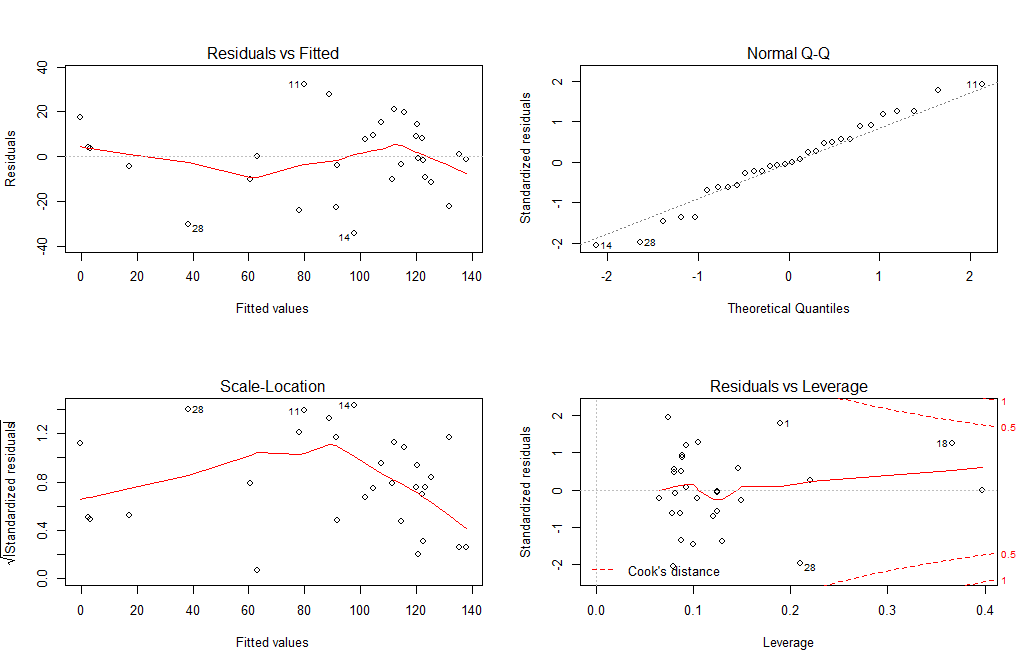
\includegraphics[scale=0.4]{imagesv2/lm_categorical_pie.png}
\caption{TFG = BUN + COL + PIE DIABETICO}
\label{fig:final_residuos}
\end{figure}

Nuestro modelo que incluye la variable Pie Diabético, cumple con el supuesto de normalidad con un p-valor de 0.8826 en el test de shapiro-wilk y con un 0.6867 en el test de Levene. Así mismo cumple con la prueba de no correlación entre los errores con un p-valor de 0.938 en el test de Durbin Watson.  

En conclusión nuestro modelo con respecto a la variable dependiente TFG asigna el coeficiente lineal de -2.0784 a la variable BUN, -0.416 a la variable Colesterol y 15.41 si el paciente cuenta con un diagnóstico de Pie Diabético neuropático. Podemos entonces definir la siguiente ecuación lineal como explicación para la variable dependiente TFG:

TFG = 185.659  -2.0784 BUN - 0.416 COL + 15.41 ( Si tenemos un diagnóstico de pie neuropático).

\section{Conclusiones}

Nuestro estudio se realizó sobre una muestra de 30 pacientes con el diagnóstico de Diabetes Mellitus, lo que constituye un factor de riesgo para desarrollar ERC, por lo que se calculó su tasa filtración glomerular (TFG), parámetro que determina el grado de enfermedad renal crónica, usando la fórmula CDK-EPI, recomendada por guías internacionales para el diagnóstico de enfermedad renal crónica. 
Existiendo en nuestra muestra un factor de riesgo establecido, como es el diagnóstico de diabetes mellitus, para desarrollar ERC, este estudio se centró en la evaluación de qué otros factores asociados en pacientes diabéticos hacen que éstos puedan o no tener daño renal, evaluado según la TFG.
La  TFG en pacientes diabéticos, según nuestro estudio se encuentra relacionada a Nitrógeno ureico sanguíneo (BUN) , ya que el 73\% del comportamiento de TFG se puede explicar por el comportamiento de BUN, con un p-value< 0.05. Asimismo la TFG asigna el coeficiente lineal de -2.0784 a la variable BUN, lo que significa que la función renal traducida por la TFG, si se  encuentra reducida, condiciona que se acumule urea en el torrente sanguíneo, incrementando el BUN. Asimismo un BUN elevado  indica un daño en la función renal, lo que se traduce en una TFG disminuida, según nuestro estudio -2.0784 a la variable BUN. Sin embargo, al no cumplir con los supuestos para una analisis de regresion lineal y a pesar de tener una alta correlación entre la variable BUN y TFG, nuestro modelo no puede explicar el comportamiento de la variable dependiente. Lo que puede explicarse debido a que la disminución en la excreción renal de urea, puede deberse a condiciones temporales como deshidratación o choque hipovolémico, consecuencia de una respuesta fisiológica a la disminución del flujo sanguíneo hacia los riñones; en este caso los valores de creatinina suelen ser normales. Recordemos que la TFG medida en los pacientes de nuestro estudio utiliza a la creatinina dentro de su fórmula CDK EPI.

El presente estudio también encontró una relación entre la TFG,  -0.4097 a la variable COL (colesterol total), lo que podría explicarse debido a que el colesterol puede acumularse en el interior de las paredes de los vasos sanguíneos. La acumulación dificulta que el corazón bombee sangre a través de los vasos y puede ocasionar ataques al corazón, derrames cerebrales y disminución de la perfusión renal. 

Nuestro modelo asociando los coeficientes de la variable BUN y COL -2.1925 y -0.4097 respectivamente, explica el 82\% de la variable TFG, aumentando significativamente la relación.

Asimismo,se encuentra una relación de 15.41 si el paciente cuenta con un diagnóstico de Pie Diabético neuropático. Este resultado se contrapone a los  escasos estudios que relacionan la tasa de filtración y el tipo de pie diabético desarrollado, como el estudio realizado por  \cite{yotsu2014comparison}, que encuentra  una menor TFG en los pacientes en los grupos isquémico y neuroisquémico en comparación con el grupo neuropático. \cite{hurley2013prospective}. examinó si la TFG sola podría ser un indicador para el cribado de pacientes de alto riesgo para úlceras por pie diabético, pero no encontró asociación entre los dos \cite{hurley2013prospective}. Sin embargo, combinar varios factores puede ayudar a aumentar la precisión de la predicción. Por ejemplo, \cite{baber2009combined}. informó que una combinación de TFG y microalbuminuria mostró una alta predictibilidad de enfermedad arterial periférica asociada a pie diabético. (Baber et al., 2009)  Estos factores son objetivos y relativamente fáciles de obtener, y por lo tanto, ideales para fines de selección,  por lo que este valor requiere mayor estudio. 
En conclusión, la diabetes y la ERC también imponen una carga económica sustancial a la sociedad, con costos particularmente altos relacionados con las complicaciones cardiovasculares y la terapia de reemplazo renal. En pacientes diabéticos niveles altos de BUN están relacionados a TFG disminuida y desarrollo de enfermedad renal crónica. La asociación de BUN elevado y colesterol alto aumenta esta relación. Se requieren  estudios más amplios para determinar la relación directa entre el tipo de pie diabético y enfermedad renal crónica.

\begin{acronym} [MPC]
\acro{TFG}{\textit{Tasa de Filtración Glomerular}}
\acro{HTA}{\textit{Diagnostico de hipertension arterial}}
\acro{GLI}{\textit{Hemoglobina Glicosilada}}
\acro{BUN}{\textit{Nitrógeno Ureico}}
\acro{HEMO}{\textit{Hemoglobina}}
\acro{COL}{\textit{Colesterol}}
\acro{ERC}{\textit{Enfermedad Renal Crónica}}
\acro{HTA}{\textit{Hipertensión Arterial}}

\end{acronym}

% Bibliography
\bibliographystyle{splncs03}
\bibliography{paper}
\end{document}

